\documentclass[10pt]{article}
\usepackage[a4paper,margin=18mm]{geometry}
\usepackage{amsmath,amssymb,graphicx,booktabs,array,xcolor}
\usepackage[hidelinks]{hyperref}
\setlength{\parindent}{0pt}
\setlength{\parskip}{5pt}
\newcommand{\F}{\mathbb F}
\newcommand{\inv}{\infty}
\begin{document}
\begin{center}
{\Large A genus-two cover of your binary elliptic curve}\\[4pt]
{\large Explicit construction and native subgroup transfer}\\
14 October 2026 \quad | \quad Run \texttt{run-20261014T1442Z}
\end{center}

For either $a=0$ or $a=1$, over the same field $k=\F_{2^{83}}$, take
\[
 E_a:\ y^2+xy=x^3+ax^2+1,\qquad
 \boxed{C_a:\ v^2+u^2v=u^5+au^4+u^3+u.}
\]
The smooth projective curve $C_a$ has genus two and a separable degree-three map
\[
 \boxed{\pi(u,v)=\left(\frac{u^3}{(u+1)^2},
 \frac{u(u+1)v+u^2+u+1}{(u+1)^3}\right).}
\]
At poles, use the projective extension: source infinity and the two geometric
points over $u=1$ map to $O$; $(0,0)$ maps to $(0,1)$.

The group law is on the abelian surface $J(C_a)$, using the homomorphism
$\pi^*:E_a\to J(C_a)$. Both curves have dimension one; $J(C_a)$ has dimension two.
All points and maps stay over $\F_{2^{83}}$. This is a same-field construction.

\begin{center}
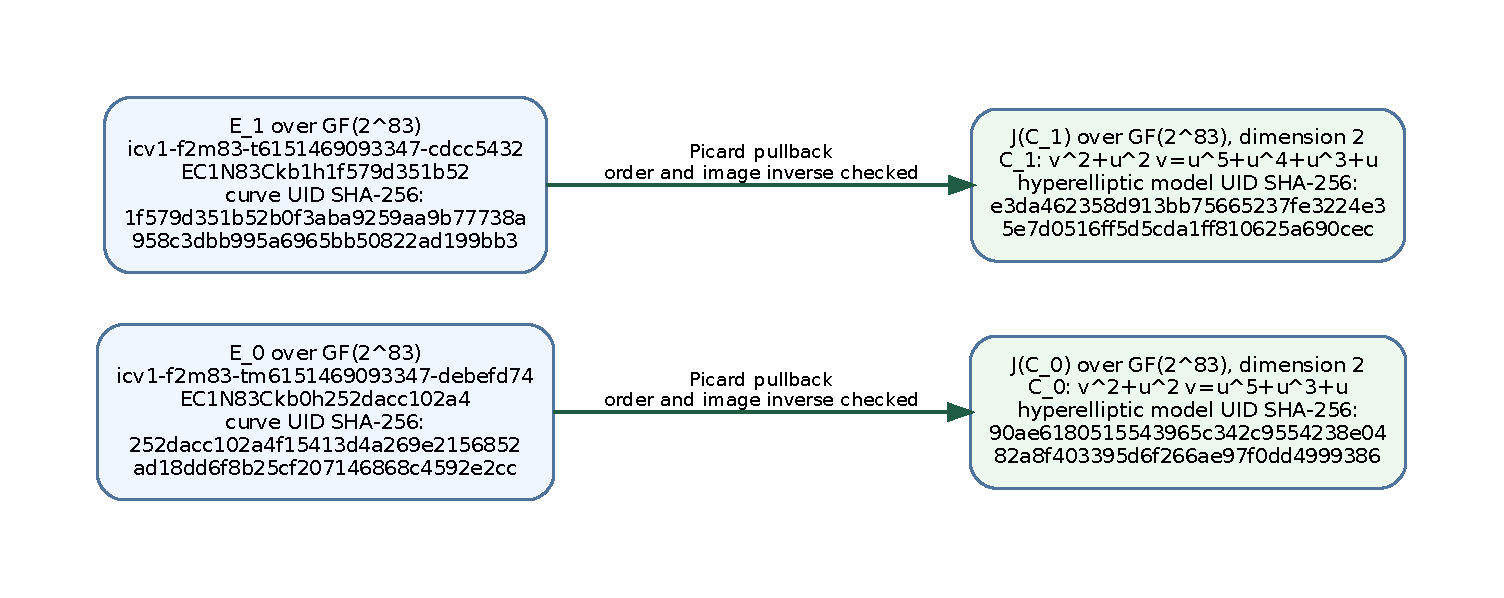
\includegraphics[width=\linewidth,height=78mm,keepaspectratio]{figures/transfer.pdf}
\end{center}
\small
The diagram gives complete source identities and target-model SHA-256 digests
(concatenate each digest's two lines). Target identifiers use
\texttt{urn:hyperelliptic-model:sha256}; they are curve-model identifiers, not EC1
subgroup identities. The cover equation and exact fields determine the models.
\normalsize

\textbf{Observed:} both pinned subgroups transfer, their generators keep their
orders, the public $Q=37P$ relation is preserved, and the image inverse recovers
both $P$ and $Q$. A faster destination solver has not been established.

\newpage
{\Large Why the construction works}

\textbf{Genus and smoothness.}
The affine equation has $v$ derivative $u^2$; at the only possible singular
point $(0,0)$ its $u$ derivative is one. At infinity, $t=1/u$, $z=v/u^3$ give
\[
 z^2+tz=t+at^2+t^3+t^5,
\]
smooth at $(t,z)=(0,0)$, with one rational point at infinity.
On $u\ne0$, set $w=v/u^2$. Then
\[
 w^2+w=u+a+u^{-1}+u^{-3}.
\]
The two Artin--Schreier poles have odd orders $3,1$, so the cover is
geometrically connected and $2g+2=(3+1)+(1+1)=6$: $g=2$.

\textbf{Equation and degree.}
Normalize $E$ by $s=(y+1)/x$, giving $s^2+s=x+a+1/x$. Write
$R=u^3/(u+1)^2$ and $s=w+1/(u+1)$. The identities
\[
 R=u+\frac{u}{(u+1)^2},\qquad
 \frac1R=\frac1u+\frac1{u^3},\qquad
 \left(\frac1{u+1}\right)^2+\frac1{u+1}=\frac{u}{(u+1)^2}
\]
prove the map equation. The degree of $R$ is three, with nonzero derivative
$u^2/(u+1)^2$. The two quadratic function-field extensions give
$[k(C):k(E)]=3$, separable. The rational map extends to the smooth projective
curves. At $u=0$ it has ramification index three; the points over $u=1$ and
source infinity map unramified to $O$.

\textbf{Explicit Jacobian transfer.}
Because $\pi^*O\sim3\inv$, for $P=(x,y)$ with $x\ne0$, the reduced pullback is
\[
 \boxed{U(u)=u^2+x^{-1}u+x,\qquad
 V(u)=\bigl(x+(y+1)x^{-2}\bigr)u+x+y+1.}
\]
Indeed the cubic fiber is $A=u^3+xu^2+x$,
$B=\kappa u^2+xu+x$, $\kappa=(y+1+x)/x$. One Cantor reduction gives
$(f+u^2B+B^2)/A=U$, $(u^2+B)\bmod U=V$.
At $O$ use $(1,0)$; at $(0,1)$ use $(u,0)$.

\textbf{Inverse and group law.}
On this image, recover $x=U(0)$, $y=V(0)+x+1$; handle $O$ and $(0,1)$
separately. Validate and reconstruct the whole pair before accepting it.
Uniqueness of reduced pairs makes this inverse injective. Picard pullback is
a homomorphism. Independently, $\pi_*\pi^*=[3]$ proves subgroup injectivity
whenever $\gcd(3,r)=1$. Both requested prime orders satisfy this condition.
A norm on arbitrary Jacobian classes is not implemented.

\newpage
{\Large Native evidence on the requested curves}

The field basis is $z^{83}+z^{45}+z^2+z+1$, modulus
\texttt{0x800000000200000000007}. Source fixtures are pinned in
\texttt{n83-final.json}. For $a=0$ the historical Sage prime receipt is reused;
for $a=1$ deterministic u64 primality is freshly checked.
\begin{center}
\begin{tabular}{crr}
\toprule $a$ & Prime subgroup order $r$ & Cofactor \\
\midrule
0 & 2417851639230796216685689 & 4\\
1 & 8569786107849059 & 1128547018\\
\bottomrule
\end{tabular}
\end{center}
For each case, native checks establish $rP=rQ=O$, valid nonzero $D_P$,
$rD_P=rD_Q=0$, inverse round trips, eight scalar relations, eight additions,
and $D_Q=37D_P$. Elliptic fixture arithmetic uses an independent u128
implementation; Jacobian arithmetic uses the existing BigUint Cantor backend.

One concrete constructed divisor, for the $a=0$ generator, is:
\begin{verbatim}
U = [0x477f77103dfad59850800, 0x34dcc667b797c42263667, 0x1]
V = [0x68da9027e8b8117caddc2, 0x14128f4ae40303ac38b16]
\end{verbatim}
Coefficients are in ascending powers. Its order is exactly the first row's
$r$, using the cited prime receipt, nonidentity and $rD_P=0$.

\begin{center}
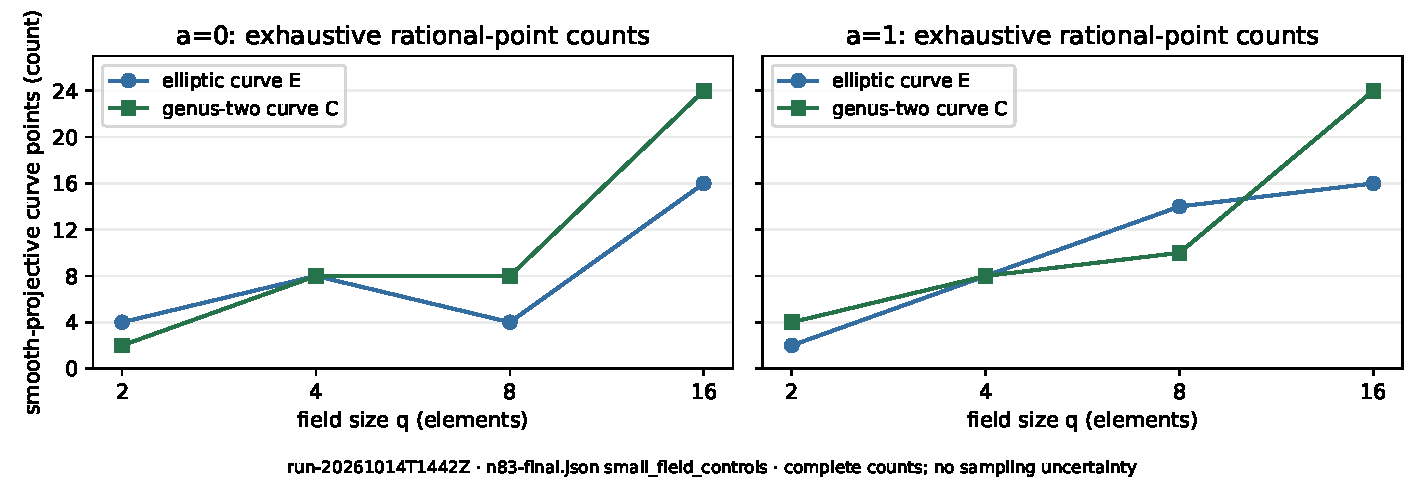
\includegraphics[width=\linewidth]{figures/counts.pdf}
\end{center}
All rational source-point maps and every ordered elliptic addition pair over
fields of sizes $2,4,8,16$ passed for both $a$ values. These are exhaustive
curve-point counts, not Jacobian orders. The plot displays recorded values
only. No field-wide scan at $2^{83}$ was attempted or required.

Negative controls reject invalid points, fields, widths and divisors; a valid
divisor outside the image; malformed CLI input; and a wrong scalar witness.
The IDC1 checker also rejects a false identity and a tampered digest.

\newpage
{\Large Proof scope and reproduction}

\textbf{Checked Lean theorem.}
Lean 4.24.0, commit
\texttt{797c613eb9b6d4ec95db23e3e00af9ac6657f24b}, with no external
dependencies, checks the actual characteristic-two affine map equation for
all field elements satisfying the source equation and $u+1\ne0$.

\begin{center}\small
\begin{tabular}{p{.40\linewidth}p{.52\linewidth}}
\toprule Declaration & Scope\\\midrule
\texttt{cleared\_map\_identity} & Cleared polynomial equality over every characteristic-two field.\\
\texttt{map\_affine\_point} & Actual inverse-denominator coordinates satisfy the elliptic equation.\\
\texttt{image\_constants\_recover\_point} & Constant-coordinate recovery equality.\\
\bottomrule
\end{tabular}\end{center}
\texttt{lake build} and the direct axiom audit pass, reporting only
\texttt{propext}, \texttt{Classical.choice}, \texttt{Quot.sound}.
No \texttt{sorryAx} occurs in the checked declarations.
\texttt{lean4checker} was not installed.

\textbf{Integration status.} Scoped package checks pass in both repositories.
The full \texttt{crypto} library suite has 4087 passes, two existing JV F4
minimum-completion failures and 117 ignored tests. Both failed tests pass
serially on the same binary. Its library source is unchanged; the full-suite
failure and unresolved cause are retained in the run's validation record.

\textbf{Partial formalization.}
Genus, projective completion, exceptional fibers, divisor-class equivalence,
Cantor correctness and Picard functoriality have the written proof on page 2
and native checks. They have not been formalized as actual geometric Lean
objects. The report's proof map and named problem retain these obligations.
The algebraic theorem is not represented as a full formal Jacobian proof.

\textbf{Identity certificate.}
\texttt{IDC1h7cbc5bff87f8b59d} checks the exact integer lift with an explicit
even correction. Native coefficient expansion agrees exactly; 32 certificate
points and 32 additional checker points pass over $2^{61}-1$. Reduction modulo
two supplies the characteristic-two identity. This is same-host evidence.

\textbf{Commands from either repository root:}
\begin{verbatim}
cargo run --release --locked \
  --manifest-path tools/binary-genus2-cover/Cargo.toml -- \
  --a both --output /tmp/genus2-n83-final.json
tools/binary-genus2-cover/check.sh
cd research/binary_genus2_cover_20261014/lean
lake build
lean BinaryGenusTwo.lean
\end{verbatim}
For supplied Q, choose one $a$, add \texttt{--q-point 0xX,0xY} and omit
\texttt{--scalar} if unknown. The scalar fields then remain null.

\textbf{Sources.} The editable Markdown report, Rust source, protocol, frozen
\texttt{n83-final.json}, exact identities, source hashes, successful validation and
failed preflights are beside this PDF. Standard geometric references:
Stichtenoth, \emph{Algebraic Function Fields and Codes}, \S3.7, and Milne,
\emph{Jacobian Varieties}. This construction supplies neither a descent to a
smaller field nor an unknown-log solution or a faster ECDLP solver.
\end{document}
